\documentclass[11pt,a4paper,fleqn]{article} 
%%%%% general %%%%%
\usepackage[T1]{fontenc} 
\usepackage{geometry}
\geometry{a4paper, top=20mm, left=20mm, right=20mm, bottom=20mm,headsep=10mm, footskip=12mm}
\usepackage[singlespacing]{setspace} %Zeilenabstand
\usepackage{xspace} %Befehle fuer Bezeichner, damit danach Leerzeichen
%%%%% lists %%%%%%

\usepackage[alwaysadjust,flushleft]{paralist}
\usepackage{enumerate}
%%%%% graphics and tables %%%%%
%\usepackage{graphicx}
\usepackage{subfigure}
\usepackage{booktabs}
\usepackage{multirow}

%\usepackage{longtable}
\usepackage{rotating}
%\usepackage{placeins}
\usepackage{flafter} %no floating object appears in the text above the position where it is defined
%\usepackage[font=small,labelfont=bf]{caption} 
\newcommand{\ra}[1]{\renewcommand{\arraystretch}{#1}}
\usepackage{tikz}
\usepackage{pgfplots}

%%%%% Mark changes %%%%%
%\usepackage{soul}
%\setstcolor{red}
%\usepackage{cancel}
\usepackage[final]{changes}

%%%%% bibliography %%%%%
\usepackage{natbib}
\bibliographystyle{abbrvnat}
\bibpunct[, ]{(}{)}{,}{a}{}{,}%
\def\bibfont{\small}%
\def\bibsep{\smallskipamount}%
\def\bibhang{24pt}%
\def\newblock{\ }%
\def\BIBand{and}%
%%%%% math and algorithms %%%%%
\usepackage{amsmath}
\usepackage{amssymb}
%\usepackage{algorithm}
\usepackage{array}
%\newcolumntype{H}{>{\setbox0=\hbox\bgroup}c<{\egroup}@{}}
\usepackage{algorithmic}
\usepackage{fixltx2e} % text super and subscripts
%%%%% color %%%%%%
\PassOptionsToPackage{usenames,dvipsnames}{color}
%\usepackage[usenames,dvipsnames]{color}
%%%%% hyperref %%%%%%
%\usepackage{url}
%\usepackage{preview}
%\usepackage{breakurl} \% break long urls
%\usepackage[colorlinks,linkcolor=Goldenrod,citecolor=Brown]{hyperref}
\usepackage{hyperref}
% \hypersetup{
%     bookmarks=true,
%     unicode=false,
%     pdftoolbar=true,
%     pdfmenubar=true,
%     pdffitwindow=false,
%     pdfstartview={FitH},
%     pdftitle={My title},
%     pdfauthor={Author},
%     pdfsubject={Subject},
%     pdfcreator={Creator},
%     pdfproducer={Producer},
%     pdfkeywords={keyword1} {key2} {key3},
%     pdfnewwindow=true,
%     colorlinks=true,
%     linkcolor=black,
%     citecolor=black,
%     filecolor=black,
%     urlcolor=black
% }


\pgfplotsset{compat=1.12}
\allowdisplaybreaks[4]
%%%%% Math Operators %%%%%
\DeclareMathOperator*{\argmin}{arg\,min}
\DeclareMathOperator*{\argmax}{arg\,max}

\usepackage{atbegshi}% http://ctan.org/pkg/atbegshi
\AtBeginDocument{\AtBeginShipoutNext{\AtBeginShipoutDiscard}}


\begin{document}

\onehalfspacing
\title{Optimizing Air Cargo Handling at an International Airline Hub for AbOvo \\ MSc Data Analytics and Decision Science RWTH Aachen University} 
\author{Ilkim Canoler \\ Luckshan Sivakumar \\  Nikhil Kulkarni \\ Karthikeyan Ramasubbu \\ Shekhar Dure}
$\newline$
$\newline$
\date{28th May 2019}
\maketitle


$\newline$
\begin{abstract}
	In this study, an operational planning problem in the air cargo industry is being tried to be solved. For all shipments in an international airline hub that need to catch their related flight on time, a mathematical model was constructed.  Working with our industrial partner AbOvo, we formalize the problem constraints and our objective. Besides, the necessary data is collected from AbOvo and we started working on it simultaneously. We are trying to establish a comprehensive view of tasks in an air cargo terminal and develop a suitable solution apporoach. Furthermore, our goal is to solve this model by using Gurobi solver as a full planning puzzle. In this paper, all explanations and details about our mathematical model and the data we have, can be found.
	
\end{abstract}

\newpage

\section{Introduction}
\label{sec:introduction}

$\newline$
An international airline hub needs to plan the air cargo movement so that all shipments catch their connecting flights or road connections. Air cargo shipments are transported in so-called unit load devices (ULDs). A ULD contains many shipments which need to go different final destinations. Hence, at the first step of the whole process, the incoming ULDs are broken down at the arrival. Here in the breakdown zone (BD), ULDs have to be unpacked and seperated. The seperate shipments are transported in the warehouse to wait for the build up call. These shipments are then moved to packing area which is called buildup zone (BU). At the end, outbound ULDs are constructed with these shipments and they are taken to the outbound flight for loading. All zones have different attributes such as number of workstations, capacities, transportation times between zones and the warehouse. Shipments also have different attributes such as priority and weight. Regarding all the attributes, constraints and the parameters which are stated in detail in problem description, the goal of the optimization process is to build up all ULDs as soon as possible to make them catching their connections.
$\newline$

$\newline$
\noindent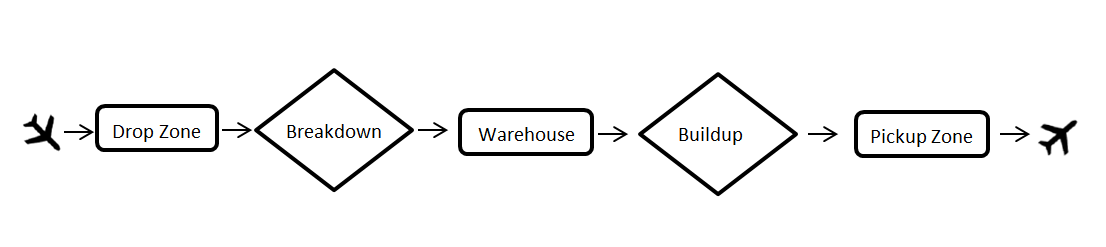
\includegraphics[width=18cm]{1_process.png}\qquad
$\newline$

\newpage

\section{Problem Description}
\label{sec:problemdescription}

$\newline$
The process of one shipment begins in drop zone when it comes to the airport in an inbound ULD. ULDs are unloaded from an aircraft by the ground handling agent and placed in a drop zone (not part of our planning puzzle). There are 4 drop zones and each drop zone has different number of workstations. Each ULD has a scheduled arrival and at a later stage an actual arrival time. From drop zone, each ULD has to be taken to the breakdown zone to get unpacked. Our problem also starts here. There are different distances between each drop zone and each breakdown zone. The sample distances between some of the drop zones and some of the BD zones are given below in the table:

$\newline$
\noindent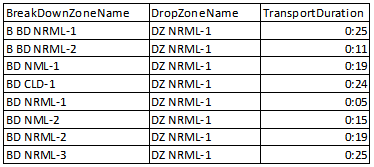
\includegraphics[width=12cm]{distances_drop_bdzone.png}\qquad

$\newline$
In BD zone, ULDs are seperated into shipments. There are 12 different BD zones in the hub. So they are located at different places of the airport. Thus all BD zones have different attributes. Attributes related to BD zones are below: 

\begin{itemize}
	\item Different characteristics for each BD zone for example some of the BD zones are for animals, some of them are for cooled products and the others are normal BD zones.
	\item Different number of workstations within the BD zone.
	\item Different transportation times to the warehouse.
	\item Different handling times per ULD.
\end{itemize}

\noindent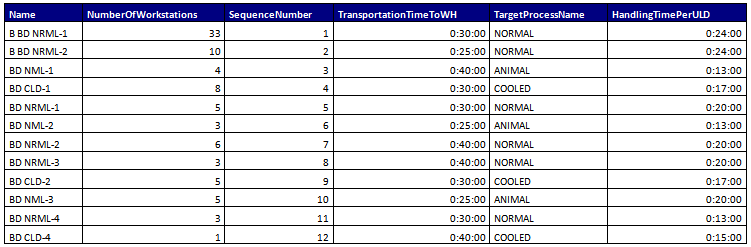
\includegraphics[width=15cm]{BDZones.png}\qquad

$\newline$
Within the BD zone, the decision needs to be taken in which order the ULDs should be unpacked. ULDs need to be broken down early enough, so all shipments can make their connections or promised pickup time. There are 3 different shipments within the hub. Cooling products, normal products (NRML) and animals (NML). Also each shipment has different priorities in these BD zones. Because some of the shipments may be animals or cooled products which are mentioned above and need to be processed before the regular shipments. ULDs contain a shipment with a high priority, need to be unpacked earlier than the others. Each shipment within the ULD is either in transit and needs to catch the connecting flight or will be further transported on the road usually by truck (not part of our planning puzzle) or is picked up from the warehouse by a customer. When the shipments are in transit and unpacked, depending on the scheduled departure time of the connection flight on which cargo is booked, it is either stored temporarily in the warehouse or directly sent to build up process. The warehouse (WH) is fully automated and with the assumption, that there are never capacity constraints in the WH. As soon as enough stock is available in the storage WH to build up one ULD for a specific aircraft, these can be requested to be provided to the BU zone.

$\newline$
In a next step the shipments are built up again to ULDs depending on their connecting flight. This is done within a build up zone (BU zone). A departing aircraft type has a link to a specific BU zone, so with the provided information which aircraft the shipment should go on, the BU zone is known. Here again a shipment with a high priority has to be built up earlier then the other shipments. There are 8 different BU zones and each BU zone has different number of workstations within. At each work station one ULD can be built up at the same time. The shipments are provided from the storage WH to the chosen work station. If the building up of two ULDs for the same aircraft are planned at one work station, it is not allowed to build up a ULD for a different aircraft in between, even if there is some idle time. The reason is that after building up one ULD there might be some shipments with the same destination left. It should be avoided to move those around, so they would stay at the work station for the build up of the next ULD for the same aircraft. From each BU zone, there are different transportation times to each flight. In addition to this, there are different default processing times for each flight which is also given in the data. This means each ULD has additional processing time before the regarding flight. Here for all ULDs, the capacity is the same which is 400 kg. For some of the flights, there is a pre-processing buffer time necessary to consider. Sample tables related to these characteristics are given below for a clear understanding:

\begin{itemize}
	\item Different handling times and transport times from the WH for each BU zone.
	
	\begin{figure}[hbt!]
		\centering
		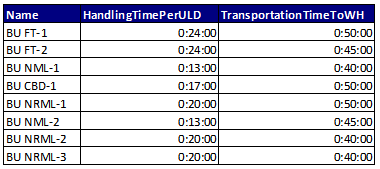
\includegraphics[width=100mm,scale=1.5]{buzone_data1.png}
	\end{figure}

\end{itemize}

	%%\noindent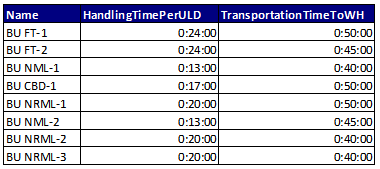
\includegraphics[width=14cm]{buzone_data1.png}\qquad

\begin{itemize}

	\item Sample workstations within some BU zones.
	
	\begin{figure}[hbt!]
		\centering
		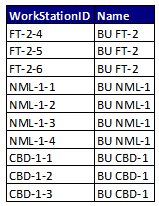
\includegraphics[width=40mm,scale=1.0]{sample_ws_bu.png}
	\end{figure}
	%%\noindent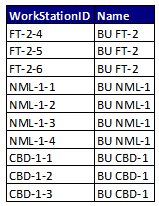
\includegraphics[width=8cm]{sample_ws_bu.png}\qquad

\end{itemize}

\begin{itemize}

	\item Sample flights related to some BU zones and the transportation time between the flight and the BU zone.
	
	\begin{figure}[hbt!]
		\centering
		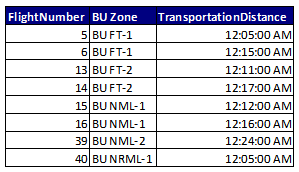
\includegraphics[width=90mm,scale=1.5]{sample_bu_flight.png}
	\end{figure}
	%%\noindent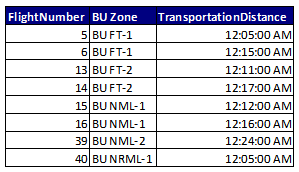
\includegraphics[width=10cm]{sample_bu_flight.png}\qquad

\end{itemize}

\begin{itemize}

	\item Pre-processing buffer times for the flights.
	
	\begin{figure}[hbt!]
		\centering
		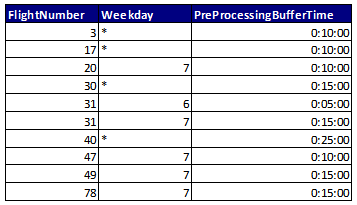
\includegraphics[width=90mm,scale=1.5]{preprocess_time.png}
	\end{figure}
	%%\noindent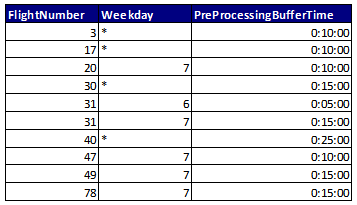
\includegraphics[width=10cm]{preprocess_time.png}\qquad
	
\end{itemize}

The goal is to build up all ULDs as soon as possible to make the connections, while the work should be processed in batches, to avoid unnecessary transportation within the BU zone.

\newpage

\section{Mathematical Model for the Problem}
\label{sec:mathmodel}

Our mathematical model for this problem is a combination of two parts of the puzzle which are Break Down Zone and the Build Up Zone. According to this, the model has different parameters, decision variables, constraints and objective function components for different zones and we treated the problem first as seperate models. At the end, overall model can be seen with both puzzles included. 

$\newline$ 

\begin{figure}[hbt!]
	\centering
	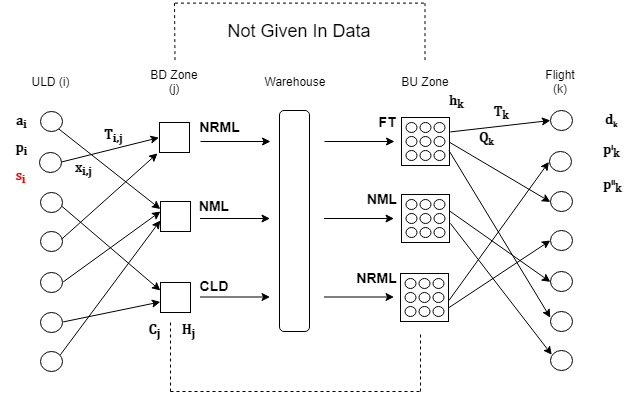
\includegraphics[width=150mm,scale=1.5]{Aircargo_overall.png}
\end{figure}


\subsection{Break Down Process}
\label{sec:ParamBDZone}

In BD zones, our model has arrival time, priority and idle time parameters for each ULD. Similar to this, each BD zone has its own capacity, handling time and transportation time from drop zone. Each ULD is a part of the ULD set I and each BD zone is a part of the BD zones set J.

\begin{equation*} ${\color{black} ULD i}$ {}  \in {}  ${\color{black}I}$ {} = {} ${\color{black}\{1,2,3,...,N\}}$  \end{equation*} 
\begin{equation*} ${\color{black} BD zone j}$ {}  \in {}  ${\color{black}J}$ {} = {} ${\color{black}\{1,2,3,...,M\}}$ \end{equation*} 


${\color{black}a_{i}}$ : Arrival time of ULD ${\color{black}i}$ in drop zone 

$\textcolor{black}{s_{i}}$ : Idle time spent by ULD ${\color{black}i}$ in drop zone

$\textcolor{black}{p_{i}}$ : Priority of ULD ${\color{black}i}$

${\color{black}c_{j}}$ : Capacity of BD zone ${\color{black}j}$

$\textcolor{black}{h_{j}}$ : Handling time in BD zone ${\color{black}j}$

$\textcolor{black}{t_{j}}$ : Time taken to transport an ULD to BD zone ${\color{black}j}$

$\newline$

\subsubsection{Decision Variable for Break Down Process}
\label{sec:DVBDZone}

In the Break Down zone, the decision needs to be taken which ULDs should be assigned to which BD zone. For this reason, the decision variable has to be binary. 1 for the ULD i is assigned to BD zone j, 0 for the ULD i is not assigned to BD zone j.

$\newline$

$\textcolor{black}{x_{ij}\in\{0,1\}, \forall {i \in I, j \in J}}$ : if a ULD i is assigned to BD zone j or not

$\newline$

\subsubsection{Constraints for Break Down Process}
\label{sec:constraintsBDZone}

For BD processes we have two constraints. The first one of them (1) is the capacity constraint and the second one (2) is the assignment constraint which means all ULDs have to be assigned to exactly one BD zone. 


\begin{align}
\sum_{i \in {I}} x_{ij} \le c_{j} \qquad \forall j \in J 
\end{align}
\begin{align}
\sum_{j \in {J}} x_{ij} = 1 \qquad \forall i \in I 
\end{align}

$\newline$

\subsubsection{Objective Function for Break Down Process}
\label{sec:objBDZone}

During the whole BD zone process, the goal is to minimize the BD zone end time for ULDs. If a ULD is assigned for the BD zone, the total time has to be calculated for that. This means total process time of one ULD i from drop zone to the end of the BD zone. For calculating this, waiting time in drop zone which is the idle time parameter, handling time and transportation time from the drop zone have to be considered if that ULD is assigned. Then we need to consider all ULDs.

$\newline$

Basically, this is the total process time for one ULD:
$\newline$

 ${\color{black}{s_{i}}}$ + ${\color{black}{t_{j}}}$ ${\color{black}{x_{ij}}}$ + ${\color{black}{h_{j}}}$ ${\color{black}{x_{ij}}}$

$\newline$
We are trying to minimize this statement above for all ULDs. Then this is the objective function for BD zone: 
$\newline$

\begin{equation*}
	\min {} \sum_{j \in J} \sum_{i \in I} (s_{i} + t_{j}x_{ij} + h_{j}x_{ij})
\end{equation*} 

%$\textcolor{black}{s_{i}}$  + ${\color{black}{t_{j}}}$ ${\color{black}{x_{ij}}}$ + ${\color{black}{h_{j}}}$ ${\color{black}{x_{ij}}}$


$\newline$

At this phase, priorities are not considered in our model in BD zones.

$\newline$

\subsection{Build Up Process}
\label{sec:ParamBUZone}

During BU process, our model has several parameters for both of the flights and the time horizons. 

\begin{equation*} ${\color{black} flight k}$ {}  \in {}  ${\color{black}K}$ {} = {} ${\color{black}\{1,2,3,...,K\}}$  \end{equation*} 
\begin{equation*} ${\color{black} time horizon t}$ {}  \in {}  ${\color{black}T}$ {} = {} ${\color{black}\{1,2,3,...,T\}}$ \end{equation*} 

The first constraint is about available weight for a given time t and for a flight k which means the summation of the weights of the seperate shipments which are raedy to build up and waiting in the warehouse.


The second one is the due time of the build up process for a flight k.

The third one is the total shipment weight as a demand for a flight k.

The fourth one is 

------------------------------------------------------------------------

\pagebreak

\begin{table}[h!]
	\begin{center}
		\caption{Drop Zone}
		\label{tab:table1}
		\begin{tabular}{l|c|c} % <-- Alignments: 1st column left, 2nd middle and 3rd right, with vertical lines in between
			\textbf{Name} & \textbf{Workstations} & \textbf{Sequence}\\
			\hline
			& & \\
			DZ NRML-1 & 6 & 1\\
			DZ NRML-2 & 4 & 2\\
			DZ NML-1 & 3 & 3\\
			DZ CLD-1 & 5 & 4\\
		\end{tabular}
	\end{center}
\end{table}

\begin{table}[h!]
	\begin{center}
		\caption{Break Down Zone}
		\label{tab:table1}
		\begin{tabular}{l|c|c|c|c} % <-- Alignments: 1st column left, 2nd middle and 3rd right, with vertical lines in between
			\textbf{Name} & \textbf{Workstations} & \textbf{Sequence} & \textbf{ToWH} & \textbf{HandTimePerULD}\\
			\hline
			& & & & \\
			B BD NRML-1 & 33 & 1 & 0:30 & 0:24\\
			B BD NRML-2 & 10 & 2 &  0:25 & 0:24\\
			BD NML-1 & 4 & 3 &  0:40 & 0:13\\
			BD CLD-1 & 8 & 4  &  0:30 & 0:17\\
			BD NRML-1 & 5 & 5  &  0:30 & 0:20\\
			BD NML-2 & 3 & 6  & 0:25 & 0:13\\
			BD NRML-2 & 6 & 7  & 0:40 & 0:20\\
			BD NRML-3 & 3 & 8  & 0:40 & 0:20\\
			BD CLD-2 & 5 & 9  & 0:30 & 0:17\\
			BD NML-3 & 5 & 10  & 0:25 & 0:20\\
			BD NRML-4 & 3 & 11  & 0:30 & 0:13\\
			BD CLD-4 & 1 & 12  & 0:40 & 0:15\\
		\end{tabular}
	\end{center}
\end{table}

\pagebreak

\textbf{\underline{\large{Arrival}}}:

Let each ULD ${\color{black}i\in{\color{black}I = \{1,2,3,\dots,n\}}}$

${\color{black}a_{i}}$ - Arrival time of each ULD ${\color{black}i}$

$\textcolor{black}{s_{i}}$ - Idle time spent by ULD i at drop zone

$\textcolor{black}{p_{i}}$ - Priority of ULD i

$\newline$

\textbf{\underline{\large{Break Down (BD) Zones}}}: $\textcolor{black}{j\in J = \{1,2,3,\dots,m\}}$

$\newline$

\textbf {From the drop zone the ULDs need to be transported to a breakdown zone (BD zone), which are located at different places of the airport, have different capacity and handling times within the zone.}

\noindent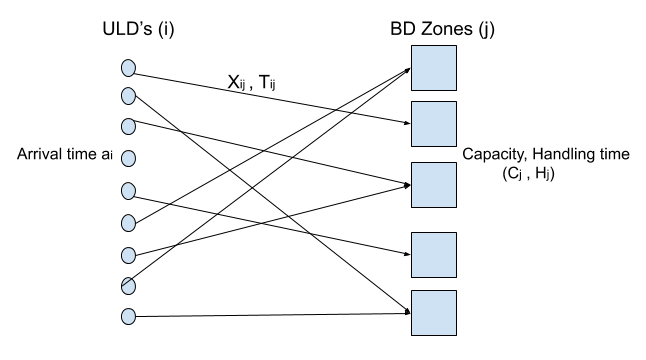
\includegraphics[width=12cm]{BDzone.png}\qquad

$\textcolor{black}{x_{ij}\in\{0,1\},\forall {i \in I, j \in J}}$ - denotes if ULD $i$ is
assigned to BD zone $j$ or not.


$\textcolor{black}{t_{j}}$ - Time taken to transport an ULD to BD
zone \textcolor{black}{$j$}

$\textcolor{black}{C_{j}}$ - Capacity of each BD Zone \textcolor{black}{$j$}

$\textcolor{black}{H_{j}}$ - Handling time of a ULD from in BD zone \textcolor{black}{$j$}

$\textcolor{black}{a_{i}+s_{i}+{\displaystyle \sum_{i,j\in E}x_{i,j}T_{j}}}$ - gives the
Arrival time of ULD \textcolor{black}{$i$} to its BD zone \textcolor{black}{$j$}

$\textcolor{black}{\displaystyle \sum_{i,j\in E}x_{i,j}}$ $\leq{C_{j}}$ , $\forall{j \in J}$ - Capacity constraint needs to be checked from time to time

\pagebreak

\textbf{\underline{\large{Warehouse}}}:

\textbf {When the shipments are unpacked, they are sent to the storage warehouse (WH) which is fully automated and with the assumption, that there are never capacity issues in the storage WH. In a next step the shipments are built up again to ULDs depending on their connecting flight. A departing aircraft type has a link to a specific BU zone, so with the provided information which aircraft the shipment should go on, the BU zone is known.
}

$\newline$

$\textcolor{black}{T_{j}^{\prime}}$ - Time taken to transport shipment from BD zone \textcolor{black}{$j$} to Warehouse

$\textcolor{black}{W_{k}}$ - Time at which, all shipments for a new Flight k are requested

$\textcolor{black}{T_{k}^{\prime}}$ - Transport time from Warehouse to BU Zone for all shipments of Flight \textcolor{black}{$k$}

$\newline$

\textbf{\underline{\large{Build Up (BU) Zone}}}:

$\newline$

$\textcolor{black}{B_{k}}$ - Time taken to Build up ALL new ULDs for flight \textcolor{black}{$k$}

$\textcolor{black}{d_{k}}$ - Departure time of a flight \textcolor{black}{$k$} must be ready (given)

$\textcolor{black}{T_{k}}$ -Transport time from BU to Flight \textcolor{black}{$k$} (given)

$\textcolor{black}{p_{k}^{\prime}}$ - Default processing time of flight \textcolor{black}{$k$} (given)

$\textcolor{black}{p_{k}^{\prime\prime}}$ - Pre processing time of flight \textcolor{black}{$k$} (given)

$\textcolor{black}{W_{k}}$ + $\textcolor{black}{T_{k}}$ +${T_{k}^{\prime}}$+ $\textcolor{black}{B_{k}}$ + $\textcolor{black}{p_{k}^{\prime}}$ + $\textcolor{black}{p_{k}^{\prime\prime}}$ $\leq$ $\textcolor{black}{d_{k}}$ //Constraint respecting Flight time

$\newline$

\noindent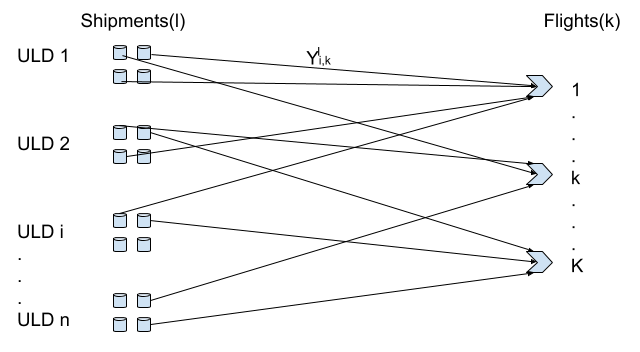
\includegraphics[width=12cm]{BUzone.png}\qquad

\pagebreak

Let $\textcolor{black}{Y_{i,k}^{l}}$ $\in\{0,1\}$ - depending on whether shipment l going to flight k is in ULD i or not.

$\textcolor{black}{w_{l}}$ - Weight of each shipment \textcolor{black}{$l$} (given)

$\textcolor{black}{Q_{k}}$ - Total weight of shipments going via flight \textcolor{black}{$k$} (summation of $\textcolor{black}{w_{l}}$)(given)

$\textcolor{black}{\displaystyle \sum_{i\in I} \sum_{l\in L}Y_{i,k}^{l}}$$\textcolor{black}{w_{l}}$ = $\textcolor{black}{Q_{k}}$ , $\forall{k}$ - Respecting assigned shipment weight to Flights \textcolor{black}{$k$}

$\textcolor{black}{\displaystyle \sum_{i\in I} \sum_{l\in L} \sum_{k\in K}Y_{i,k}^{l}}$ - N // Total no of shipments

All shipments of flight k, should reach be available before time $\textcolor{black}{W_{k}}$:

$\textcolor{black}{a_{i}+s_{i}+{\displaystyle \sum_{i,j\in E}x_{i,j}T_{j}}}+{T_{j}^{\prime}}+{H_{j}}$ $\leq$ ${W_{k}}$ + (1-${Y_{i,k}^{l}}$)M, $\forall{i,k,l}$ // Time constraint for every shipment.

$\newline$

\textbf{\large{Objective Function}}: Minimizing the maximum slack
$\newline$

$\textcolor{black}{Min(Max(  s_{i}}+{W_{k}}$))

\end{document}